\subsection{可逆双模与森田等价}

定义 1. —— 设 A 与 B 是 k-代数，P 是一个 \((\mathrm{A},\mathrm{B})_{k}\)-双模。若存在一个 \((\mathrm{B},\mathrm{A})_{k}\)-双模 Q，使得 \(P \otimes_{B} Q\) 同构于 \(_{s}A_{d}\) 且 \(Q \otimes_{A} P\) 同构于 \(_{s}B_{d}\)，则称 P 是可逆的。这样的双模 Q 称为 P 的逆。

设 A 与 B 是 k-代数，P 是一个可逆 \((\mathrm{A},\mathrm{B})_{k}\)-双模。设 C 是一个 k-代数，\(P'\) 是一个可逆 \((\mathrm{B},\mathrm{C})_{k}\)-双模。最后，设 Q 与 \(Q'\) 分别是 P 与 \(P'\) 的逆双模。由张量积的结合性（II, §3, No.~8, 第 258 页，命题 8）及 II, §3, No.~4, 第 249 页的命题 4，\((\mathrm{C},\mathrm{A})_{k}\)-双模 \(Q'\otimes_{B}Q\) 是 \((\mathrm{A},\mathrm{C})_{k}\)-双模 \(P\otimes_{B}P'\) 的一个逆，因而 \(P\otimes_{B}P'\) 是可逆 \((\mathrm{A},\mathrm{C})_{k}\)-双模。于是，关系

“A 与 B 是 k-代数，且存在一个可逆 \((A,B)_{k}\)-双模”是一个等价关系。

定义 2. —— 若存在一个可逆 \((\mathrm{A},\mathrm{B})_{k}\)-双模，则称两个 k-代数 A 与 B 是森田等价的。若 Z-代数 A 与 B 是森田等价的，则称环 A 与 B 是森田等价的。

两个同构的 k-代数是森田等价的。若两个 k-代数森田等价，则它们的反代数也森田等价。

设 P 是一个可逆 \((\mathrm{A},\mathrm{B})_{k}\)-双模，Q 是 P 的一个逆。则 Q 是可逆 \((\mathrm{B},\mathrm{A})_{k}\)-双模，且以 P 为逆。此外，把 P 视为 \((\mathrm{B}^{\circ},\mathrm{A}^{\circ})_{k}\)-双模时，P 是可逆的，且以 \((\mathrm{A}^{\circ},\mathrm{B}^{\circ})_{k}\)-双模 Q 为逆。

引理 1. —— 设 A 与 B 是 k-代数，P 是一个可逆 \((\mathrm{A},\mathrm{B})_{k}\)-双模，M 与 N 是 B-模，\(u:M\to N\) 是一个 B-线性映射。若映射 \(1_{P}\otimes u:P\otimes_{B}M\to P\otimes_{B}N\) 为零（相应地，为双射），则 u 亦然。

设 Q 是 P 的逆双模，\(\theta: Q \otimes_{A} P \to_{s} B_{d}\) 是一个 \((B, B)_{k}\)-双模同构。本引理由下述图式的交换性得出

\pandocbounded{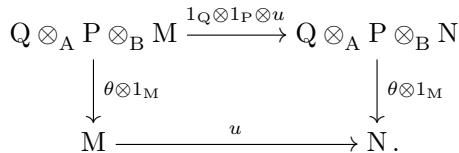
\includegraphics[keepaspectratio]{images/part001_2598f5b2.jpg}}

定理 1. —— 设 A 与 B 是 k-代数，P 是一个 \((A,B)_{k}\)-双模。把 \((B,A)_{k}\)-双模 \(\operatorname{Hom}_{\mathrm{A}}(\mathrm{P},\mathrm{A}_{s})\) 记作 \(P^{*}\)。下列性质等价：

\begin{enumerate}
\def\labelenumi{(\roman{enumi})}
\item
  \((\mathrm{A},\mathrm{B})_k\)-双模 P 是可逆的。
\item
  A-模 P 是投射的、有限生成的且是生成模，且映射 \(b \mapsto b_{P}\)（从 B 到 \(\operatorname{End}_{\mathrm{A}}(\mathrm{P})^{\circ}\)）是 k-代数同构。
\item
  右 B-模 P 是投射的、有限生成的且是生成模，且映射 \(a \mapsto a_{P}\)（从 A 到 \(\operatorname{End}_{\mathrm{B}}(\mathrm{P})\)）是 k-代数同构。若这些性质成立，则同态
\end{enumerate}

\[
\Theta : \mathrm{P} ^ {*} \otimes \mathrm{P} \to {} _ {s} \mathrm{B} _ {d} \quad \text{且} \quad \Lambda : \mathrm{P} \otimes \mathrm{P} ^ {*} \to {} _ {s} \mathrm{A} _ {d}
\]

均为同构，于是 \((\mathrm{B},\mathrm{A})_k\)-双模 \(\mathrm{P}^*\) 是 \(\mathrm{P}\) 的一个逆。

若性质 (ii) 成立，则 P 是一个可逆 \((\mathrm{A},\mathrm{B})_{k}\)-双模，其逆为 \(P^{*}\)（VIII, 第 98 页，命题 2 及第 98 页，命题 3）。这就证明了 (ii) 蕴含 (i) 以及最后一个断言。

设 \((\mathrm{A},\mathrm{B})_{k}\)-双模 P 是可逆的。那么 A-模 P 是生成模（VIII, 第 98 页，命题 3, (iii) \(\Rightarrow\) (i)）。因而它是忠实的且平衡的（VIII, 第 82 页，定理 2），于是映射 \(a \mapsto a_{p}\)（从 A 到 \(\operatorname{End}_{\mathrm{B}}(\mathrm{P})\)）是双射。

现在证明映射 \(b \mapsto b_{\mathrm{P}}\)（从 B 到 \(\mathrm{End}_{\mathrm{A}}(\mathrm{P})\)）是双射。设 Q 是一个 \((\mathrm{B},\mathrm{A})_k\)-双模，它是 P 的逆。设 \(u \in \mathrm{End}_{\mathrm{A}}(\mathrm{P})\)；则 \(1_{\mathrm{Q}} \otimes u\) 是左 B-模 \(\mathbf{Q} \otimes_{\mathrm{A}} \mathbf{P}\) 的一个自同态。由于 \((\mathrm{B},\mathrm{B})_k\)-双模 \(\mathbf{Q} \otimes_{\mathrm{A}} \mathbf{P}\) 同构于 \({}_s\mathbf{B}_d\)，存在 B 中唯一的元素 \(b\)，使得 \(1_{\mathrm{Q}} \otimes u\) 是以 \(b\) 为比的、右 B-模 \(\mathbf{Q} \otimes_{\mathrm{A}} \mathbf{P}\) 的位似。于是我们有 \(1_{\mathrm{Q}} \otimes (u - b_{\mathrm{P}}) = 0\)。从而由引理 1 得 \(u = b_{\mathrm{P}}\)；这就证明了映射 \(b \mapsto b_{\mathrm{P}}\)（从 B 到 \(\operatorname{End}_{\mathrm{A}}(\mathrm{P})\)）是双射。

于是由 VIII, 第 98 页的命题 2，A-模 P 是投射的且有限生成的。这样我们就证明了 (i) 与 (ii) 的等价性。

交换 A 与 B 的角色，即得 (i) 与 (iii) 的等价性，命题证毕。

推论 1. —— 设 A 与 B 是森田等价的 k-代数，P 是一个可逆 \((A,B)_{k}\)-双模。存在一个同构 \(\varphi\)，从 A 的中心 \(Z(A)\) 到 B 的中心，它由关系式 \(\varphi(z)_{\mathrm{P}} = z_{\mathrm{P}}\)（对每个 \(z \in Z(A)\)）确定。\((A,B)_{k}\)-双模 P 的自同构是诸位似 \(z_{P}\)，其中 z 是 \(Z(A)\) 的一个可逆元素。

给定定理 1，这由 VIII, 第 97 页的注 2 得出。

推论 2. —— 设 A 与 B 是森田等价的 k-代数，P 是一个可逆 \((\mathrm{A},\mathrm{B})_{k}\)-双模。每个与 P 互逆的 \((\mathrm{B},\mathrm{A})_{k}\)-双模都同构于 P 的对偶 \(\mathrm{P}^{*}=\mathrm{Hom}_{\mathrm{A}}(\mathrm{P},\mathrm{A})\)。更精确地说，设 Q 是一个作为 P 的逆的 \((\mathrm{B},\mathrm{A})_{k}\)-双模，\(\lambda:P\otimes_{B}Q\to_{s}A_{d}\) 是 \((\mathrm{A},\mathrm{A})_{k}\)-双模的一个同构。存在唯一的映射 \(\tau:\mathrm{Q}\to\mathrm{P}^{*}\)，它由关系式 \(\langle p,\tau(q)\rangle=\lambda(p\otimes q)\)（\(p\in P\)，\(q\in Q\)）确定，且 \(\tau\) 是 \((\mathrm{B},\mathrm{A})_{k}\)-双模的同构。

映射 \(\tau\) 的存在性与唯一性是明显的。它是 \((\mathrm{B},\mathrm{A})_{k}\)-双模的同态，并且我们有 \(\lambda=\Lambda\circ(1_{\mathrm{P}}\otimes\tau)\)。由于 \(\lambda\) 与 \(\Lambda\) 都是 \((\mathrm{A},\mathrm{A})_{k}\)-双模的同构（VIII, 第 101 页，定理 1），\(1_{P}\otimes\tau\) 亦是。由引理 1，映射 \(\tau\) 是双射。

注. —— 在该推论的假设下，设 q 是 Q 的一个元素，使得 \(\lambda(p \otimes q) = 0\)（对每个 \(p \in P\)）。那么我们有 \(\tau(q) = 0\)，即 q = 0。同样，若 p 是 P 的一个元素，使得 \(\lambda(p \otimes q) = 0\)（对每个 \(q \in Q\)），则 p = 0。

例. —— 1) 设 B 是一个 \(k\)-代数，\(n\) 是一个 \(\geqslant 1\) 的整数，A 是 \(k\)-代数 \(\mathbf{M}_n(\mathrm{B})\)。右 B-模 \(\mathrm{P} = \mathrm{B}_d^n\) 是投射的、有限生成的且是生成模，并且 A 可以等同于 P 的自同态代数（II, §10, No.~7, 第 349 页）。由定理 1，\((\mathrm{A},\mathrm{B})_k\)-双模 P 是可逆的。于是代数 B 与 \(\mathbf{M}_n(\mathrm{B})\) 是森田等价的。

\begin{enumerate}
\def\labelenumi{\arabic{enumi})}
\setcounter{enumi}{1}
\tightlist
\item
  *设 A 是一个交换 \(k\)-代数，P 是一个 A-模。我们把 P 视为一个两个作用律相等的 \((A, A)_k\)-双模。若 \((A, A)_k\)-双模 P 是可逆的，则 A-模 P 是有限生成的（定理 1）。由《交换代数》II, §5, No.~4, 第 114 页的定理 3，下列性质等价：
\end{enumerate}

\begin{enumerate}
\def\labelenumi{(\roman{enumi})}
\item
  \((\mathrm{A},\mathrm{A})_{k}\)-双模 P 是可逆的。
\item
  存在一个 A-模 \(\mathrm{Q}\)，使得 \(\mathrm{P} \otimes_{\mathrm{A}} \mathrm{Q}\) 同构于 \(\mathrm{A}\)。
\item
  A-模 P 是投射的、有限生成的，且秩为 1。 *
\end{enumerate}

